\documentclass[12pt]{article}
\usepackage[utf8]{inputenc}
\usepackage[T1]{fontenc}
\usepackage[brazil]{babel}
\usepackage{graphicx}
\usepackage{geometry}
\usepackage{float}
\geometry{a4paper, left=3cm, right=2cm, top=3cm, bottom=2cm}

\begin{document}

\begin{center}
    \LARGE\textbf{Relatório Técnico: Educação e Crescimento Econômico}
\end{center}

\section{Introdução}
Este relatório apresenta uma análise da relação entre investimento em educação e crescimento econômico com base em dados do Banco Mundial.

\section{Resultados}
\begin{figure}[H]
    \centering
    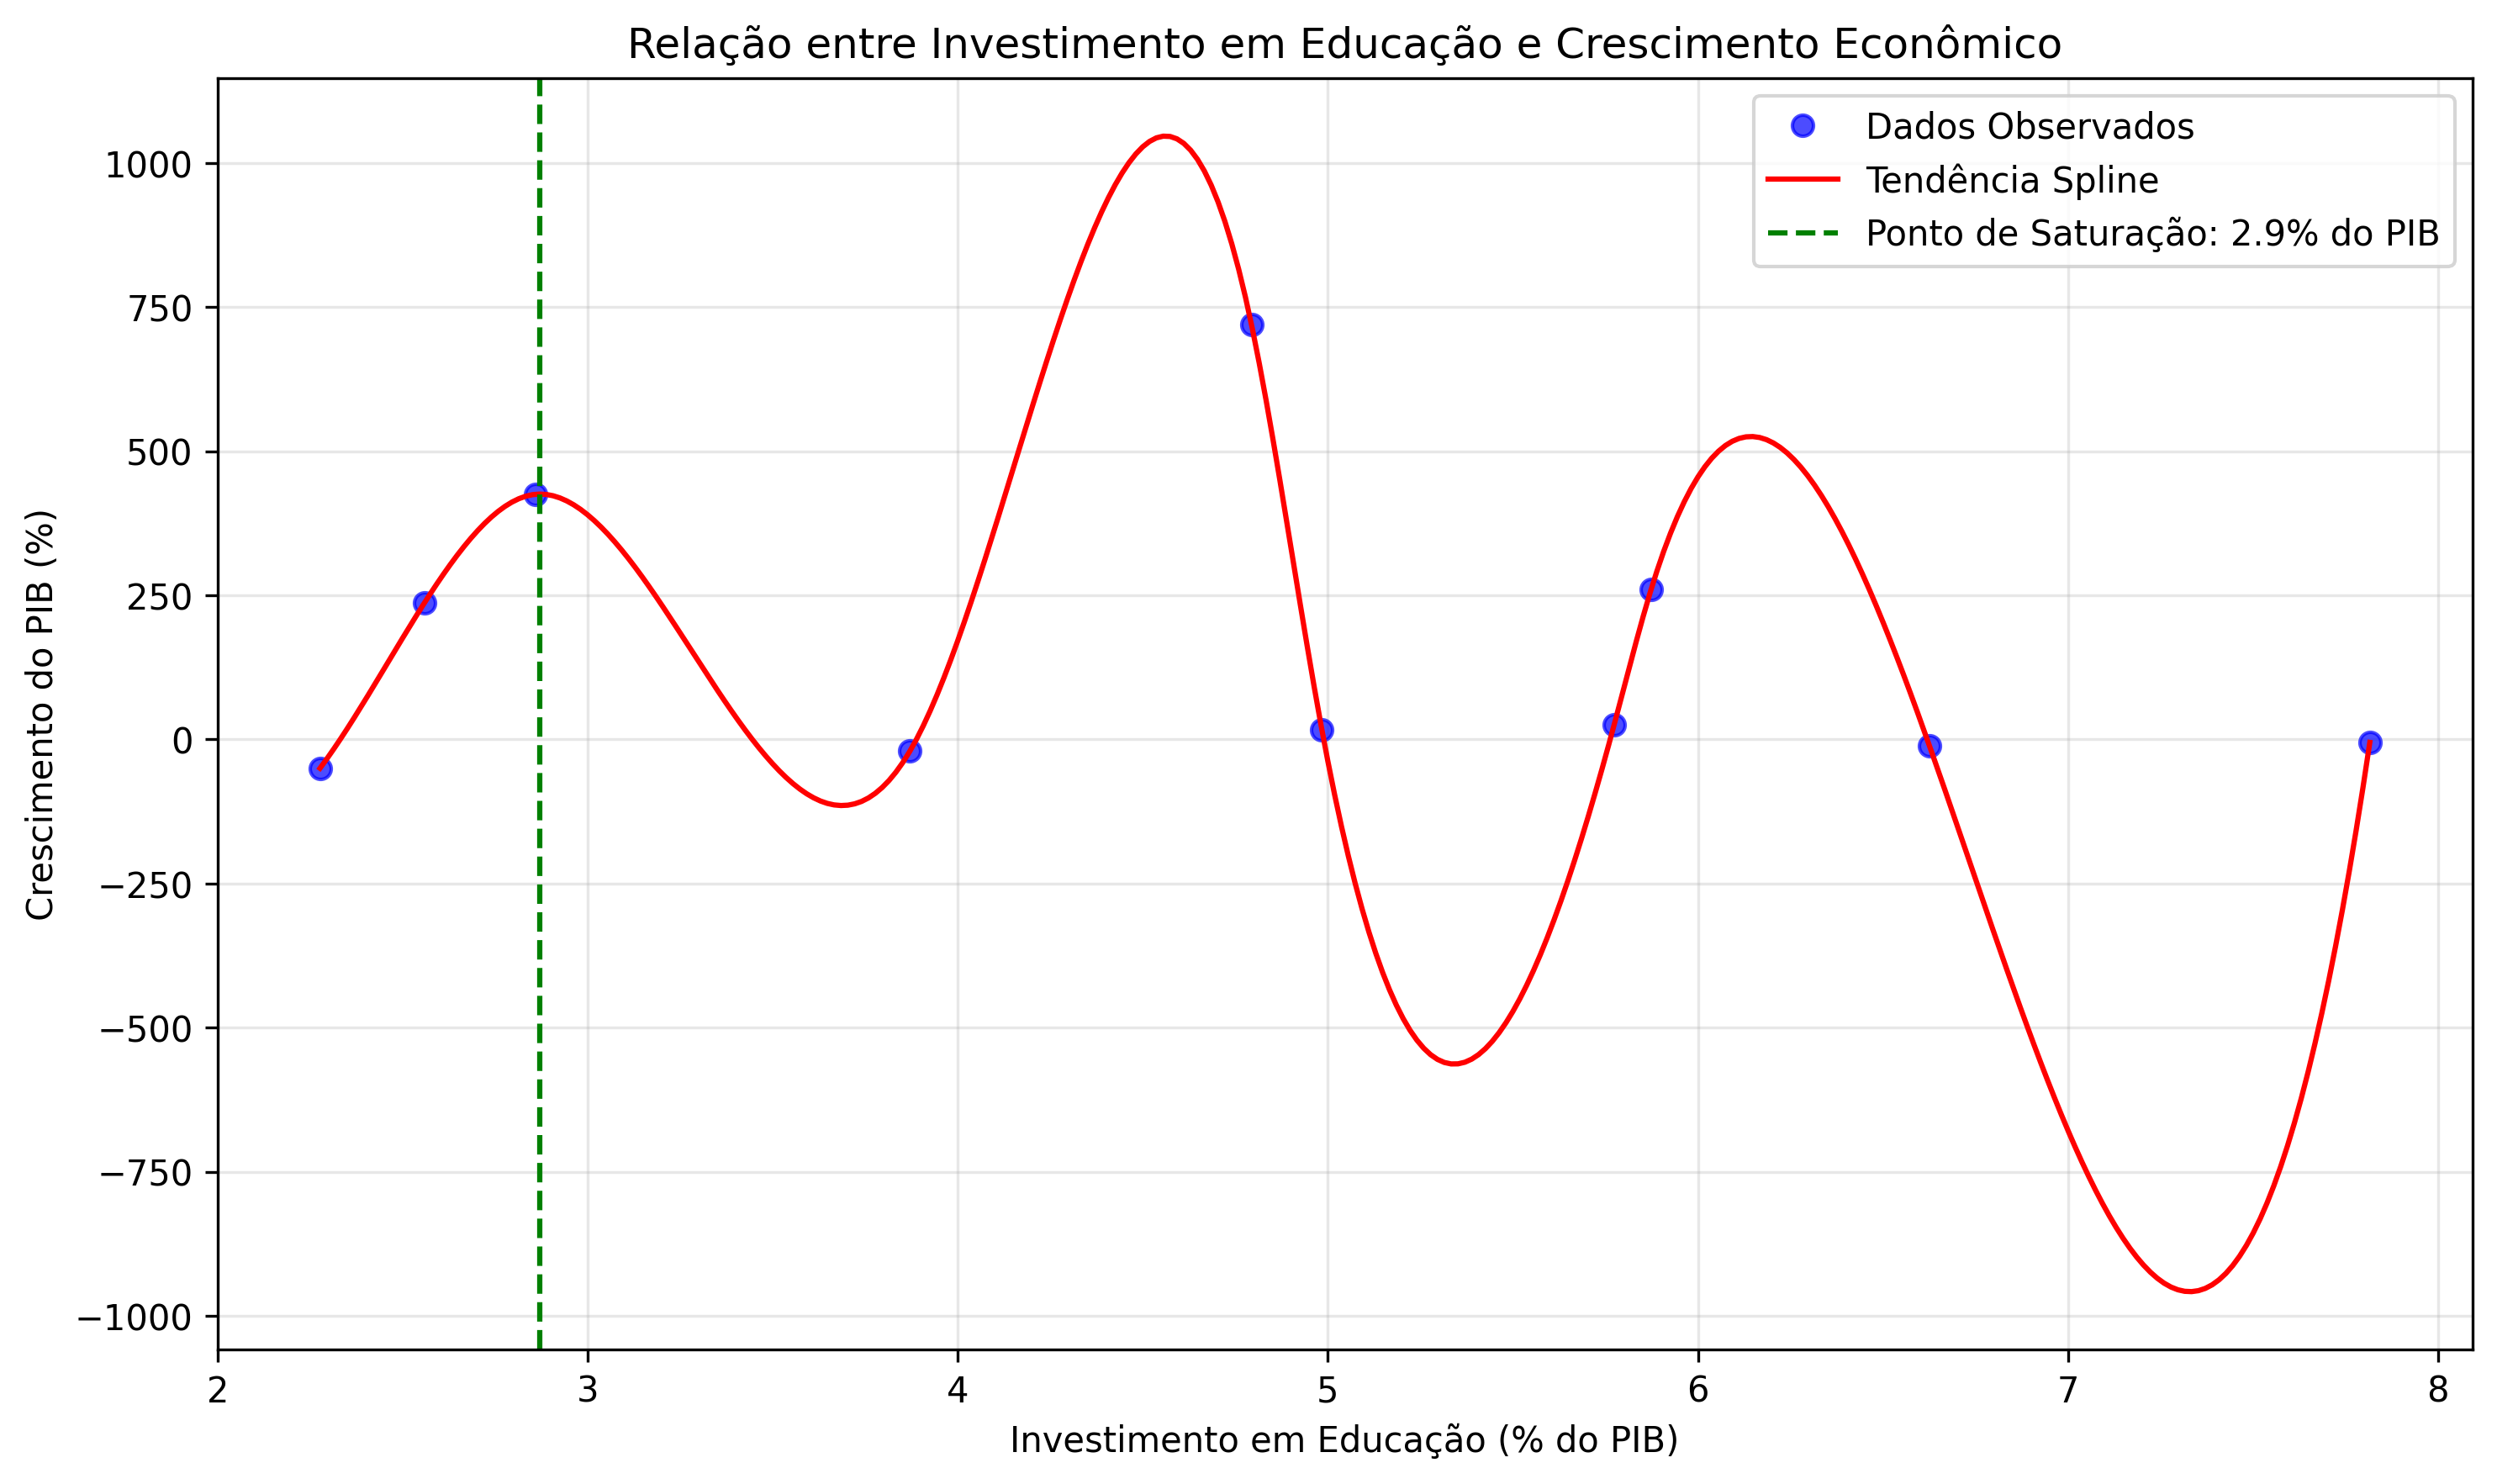
\includegraphics[width=0.9\textwidth]{relacao_educacao_crescimento.png}
    \caption{Investimento em educação vs Crescimento do PIB}
\end{figure}

\subsection{Métricas Principais}
\begin{itemize}
    \item Correlação global: -0.205
    \item Ponto de saturação: 2.9\% do PIB
\end{itemize}

\end{document}